\chapter{یادگیری با نمونه}
\label{chap:two}
همانطور که در پیش‌گفتار بحث شد، فرآیند یادگیری نیازمند نمونه‌داده‌هایی است که بتوانیم به وسیله آن‌ها مدل را آموزش دهیم  و بتوانیم داده‌های حدید را دسته بندی کنیم. در این فصل روش‌هایی که برای دسته‌بندی داده‌های جدید به نمونه نیاز دارند بررسی می‌شوند و یک مثال از یادگیری با یک نمونه برای فهم بهتر مبحث آورده شده‌است.

در یادگیری به صورت سنتی، باید داده‌ها با دو دسته آموزش و آزمون تقسیم‌بندی شوند و برای هر کلاس جدید برای دسته‌بندی باید به تعداد کافی داده وجود داشته باشد تا مدل بتواند دسته‌بندی مناسبی انجام دهد. مانند مدل کانولوشن ساده‌ای که با آن می‌توان سگ و گربه را از هم تفکیک داد. این مدل برای هر داده سگ و گربه باید تعداد قابل توجهی داده دیده باشد تا بتواند دسته‌بندی را به درستی انجام دهد. حال برای دسته‌بندی یک حیوان دیگر توسط این مدل باید داده‌های جدیدی به مدل بدهیم تا مدل بتواند آن نوع حیوان را نیز دسته‌‌بندی کند.

با بهبود ساختار شبکه یادگیرنده می‌توان نیاز فرآیند یادگیری به داده‌های زیاد را کاهش داد تا مدل بتواند با داده‌های کم نیز دسته‌بندی را انجام دهد. ارائه راهکار‌ها و روش‌هایی در کنار استفاده از شبکه‌های عصبی این امکان را به وجود آورد تا مدل فقط با دیدن یک نمونه از یک کلاس داده در فرآیند آموزش بتواند داده جدید را دسته‌بندی کند. این روش با نام یادگیری با یک نمونه شناخته می‌شود.

در این روش در فرآیند آموزش مدل به حداقل یک داده از یک کلاس داده نیاز دارد. برای جلوگیری از 
\trans{بیش‌برازش}{over fitting}
 در فرآیند آموزش از روش‌هایی مانند ایجاد اعوجاج در داده‌ها برای تولید داده جدید در حالات مختلف استفاده می‌شود تا مدل بتواند دسته‌بندی بهتری انجام دهد. فرآیند یادگیری با یک نمونه در مواردی پر کاربرد تر است که ما تمامی کلاس‌های داده را از قبل داشته‌باشیم؛ برای مثال: در مبحث پردازش زبان طبیعی انسان، ساختار هر زبان مشخص است و زبان‌ها از یکدیگر با ساختار‌های مشخص قابل تفکیک هستند و هر زبان تعداد ثابتی قواعد و واژگان دارد. این قابلیت به ما کمک می‌کند تا بتوانیم از مدل یادگیری با یک نمونه برای کاربرد پردازش زبان طبیعی استفاده کنیم. با یک مثال و بررسی یک ساختار شبکه ارائه شده در یک مقاله به بررسی بیشتر این موضوع می‌پردازیم. 
 
 زبان سیامی یکی از زبان‌های آسیایی است و ساختار مشخص و واژگان ثابتی را دارد. در ادامه قصد داریم با معرفی یک مدل بتوانیم واژگان دست‌نویس این زبان  را تفکیک و دسته‌بندی کنیم.
 
 \section{مدل}
 مدل به صورت یک شبکه عصبی دو قلو است. برای دسته‌بندی این شبکه دوتایی‌های مشابه و مخالف را ایجاد می‌کند. یعنی با استفاده از شباهت‌ها و تفاوت‌های موجود درون کاراکترهای زبان آن‌ها را دسته‌بندی می‌کند در انتها هنگام دریافت نمونه جدید شبکه شباهت و تفاوت‌های این نمونه با نمونه‌های موجود را تشخیص می‌دهد و آن را در یک دسته قرار می‌دهد.
 
برای محاسبه تفاوت و شباهت یک معیار فاصله وزن دار L1 بین بردار‌های ویژگی استخراج شده از دو شبکه دو قلو استفاده کرده و بر اساس آن نرخ یادگیری شبکه و نحوه دسته‌بندی واژگان را مشخص کرده‌است. در شکل
\ref{report:simple binarry siamese}
یک نمونه ساده از این شبکه برای دسته بندی دودویی را مشاهده می‌کنید.
 
%\newpage
\begin{figure}[h]
	\centering
	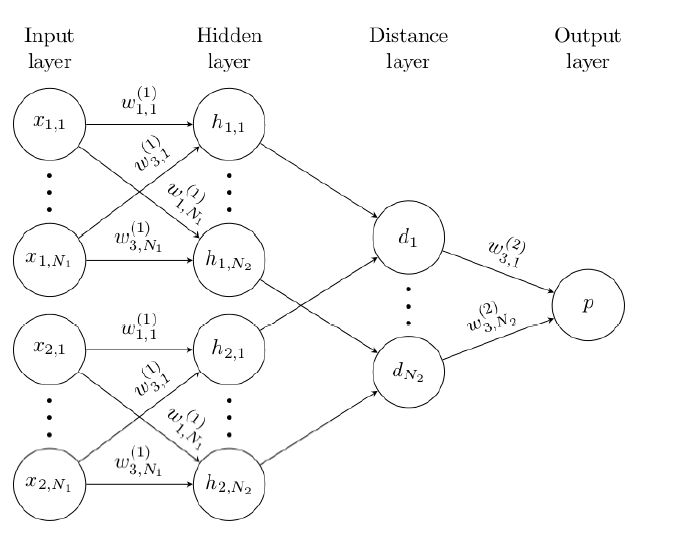
\includegraphics[width=0.5\textwidth]{img/report/simple_binary_classification_siamese}
	\caption{شبکه ساده سیامی برای دسته بند دودویی \cite{Koch}}
	\label{report:simple binarry siamese}
	\centering
\end{figure}

همانطور که گفتیم این شبکه ساختاری دو قلو دارد که بتواند یک زوج مشابه یا متفاوت را دسته بندی کند. ساختار یک نیمه از این شبکه را در شکل 
\ref{report:siamese half network}
مشاهده می‌کنید.
\begin{figure}[h]
	\centering
	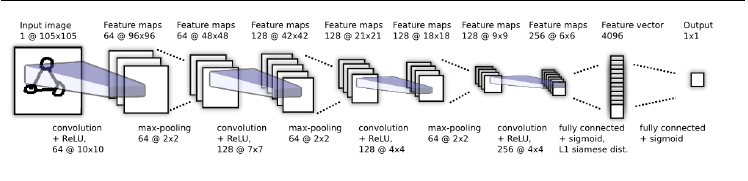
\includegraphics[width=0.9\textwidth]{img/report/siamse_half_network}
	\caption{یک نیمه از شبکه دو قلو استفاده شده \cite{Koch}}
	\label{report:siamese half network}
	\centering
\end{figure}

با توجه به اینکه دادگان کمی برای آموزش در اختیار است، برای جلوگیری از بیش‌برازش داده‌های موجود در حالات مختلف اعوجاج داده شده‌اند. اعوجاج داده این کمک را می‌کند تا با نمونه‌های حتی اندک هم بتوانیم دسته‌بندی مناسبی ارائه کنیم.
\ref{report:augmented siamese data}

\begin{figure}[h]
	\centering
	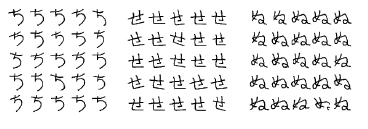
\includegraphics[width=0.6\textwidth]{img/report/augmented_siamese_data}
	\caption{دادگان اعوجاج داده شده \cite{Koch}}
	\label{report:augmented siamese data}
	\centering
\end{figure}
\section{دادگان}
دادگان استفاده شده 
\lr{Omniglot}
است. این دادگان شامل نمونه‌هایی از ۵۰ الفبای مختلف است. به سه صورت همانطور که در جدول 
\ref{report:omniglot verification siamese}
 مشاهده می‌کنید از این دادگان استفاده شده‌است و دقت مرحله 
 \trans{تایید}{verification} 
 را در جدول آورده است.

\begin{table}[h]
	\begin{center}
	 	\caption{دقت مرحله تایید در سه دسته انتخاب دادگان  \cite{Koch}}
		\begin{tabular}{cl}
			
			\hline Method & Test \\
			\hline \lr{$30 \mathrm{k}$ training }& \\
			\lr{$n o$ distortions }& 90.61 \\
			\lr{affine distortions $\mathrm{x} 8$} & 91.90 \\
			\lr{$90 \mathrm{k}$ training }& \\
			\lr{$n o$ distortions} & 91.54 \\
			\lr{affine distortions $\times 8$ }& 93.15 \\
			\lr{$150 \mathrm{k}$ training} & \\
			\lr{$n o$ distortions} & 91.63 \\
			\lr{affine distortions $\mathrm{x} 8$ }& 93.42 \\
			\hline
		\end{tabular}

	 	\label{report:omniglot verification siamese}
	\end{center}
\end{table}
در مقایسه با این روش‌، روش‌های دیگری نیز تعریف شده‌اند که صرف نظر از دقت انسان بهترین آن‌هامدل بر پایه روابط احتمالاتی و در رتبه بعد این روش جزو بهترین روش‌های ارائه شده برای دسته‌بندی واژگان است. روش‌های دیگر در 
\ref{report:method_compare_siames}

\begin{table}[h]
	\begin{center}
		\caption{مقایسه روش‌‌های مختلف \cite{Koch}}
		\begin{tabular}{rr}
			\hline Method & Test \\
			\hline Humans & 95.5 \\
			\lr{Hierarchical Bayesian Program Learning} & 95.2 \\
			\lr{Affine model} & 81.8 \\
			\lr{Hierarchical Deep} & 65.2 \\
			\lr{Deep Boltzmann Machine} & 62.0 \\
			\lr{Simple Stroke} & 35.2 \\
			\lr{1-Nearest Neighbor} & 21.7 \\
			\lr{Siamese Neural Net} & 58.3 \\
			\lr{Convolutional Siamese Net} & 92.0 \\
			\hline
		\end{tabular}

		\label{report:method_compare_siames}
\end{center}
\end{table}


در پایان برای نشان‌ دادن قدرت شبکه و عام بودن استفاده از آن، دادگان MNIST انتخاب شده است و بر روی این دادگان که حاوی کاراکتر‌های دست‌نویس است این مدل با مدل 
\lr{1-nearest neighbor}
 مقایسه شده است، دقت بسیار بالاتری را کسب کرده است اما برای این دادگان کافی نیست و هدف نشان دادن این بوده‌است که این روش و شبکه را می‌توان با اصلاحاتی برای استفاده‌های دیگر نیز طراحی و آماده کرد. همان‌طور که در جدول
 \ref{report:siamese_vs_1NN}
 مشاهده می‌کنید روش یادگیری با یک نمونه به راحتی قابل تعمیم است و می‌توان از آن برای حل مسائل مختلف استفاده کرد.


\begin{table}[h]
	\begin{center}
		\caption{مقایسه با 1NN \cite{Koch}}
		\begin{tabular}{cc}
			\hline Method & Test \\
			\hline \lr{1-Nearest Neighbor} & 26.5 \\
			\lr{Convolutional Siamese Net} & 70.3 \\
			\hline
		\end{tabular}
		\label{report:siamese_vs_1NN}
	\end{center}
\end{table}

 
\section{سخن پایانی}
در این فصل سعی شد تلاش صورت گرفته برای کاهش وابستگی مدل به داده و یادگیری با نمونه و انواع آن را با بررسی یک مقاله در حوزه یادگیری با یک نمونه توضیح دهیم.

